\section{Introduction}
\label{s:intro}

%\wajih{I have updated the macro logs as it does not make sense to use \ logs for just "system". I have changed the macro to "system logs". Make sure the paper is consistent with that.}

% The effectiveness of IDSes hinges on their ability to accurately detect these threats, maintain low false positive rates, and operate with minimal resource consumption, ensuring system performance is not compromised.

%\wajih{Give the workflow of MSSP and cite that organizations outsource their security. If you find any numbers on how many comapnies use MSSP and outsource their security operations that would be great. If you find any realworld attack examples on MSSP where the data was leaked that would be great as well. }

Intrusion Detection Systems (\ids) are crucial for countering Advanced Persistent Threats (APTs) in enterprises, as evidenced by major attacks, such as Solar Winds~\cite{solarwinds} and NotPetya~\cite{notpetya}. Given their stealth and persistence, many enterprises rely on Managed Security Service Providers (MSSPs) to improve their defenses. A survey~\cite{msspsurvey} involving over 5,000 IT professionals reported that about 75\% of companies use MSSPs. These providers integrate their security systems with clients' systems to manage \logs, typically configuring the clients' systems to transmit \logs to the cloud for analysis. Figure~\ref{mssp} illustrates this MSSP operational architecture.


\begin{figure}[t!]
  \centering
  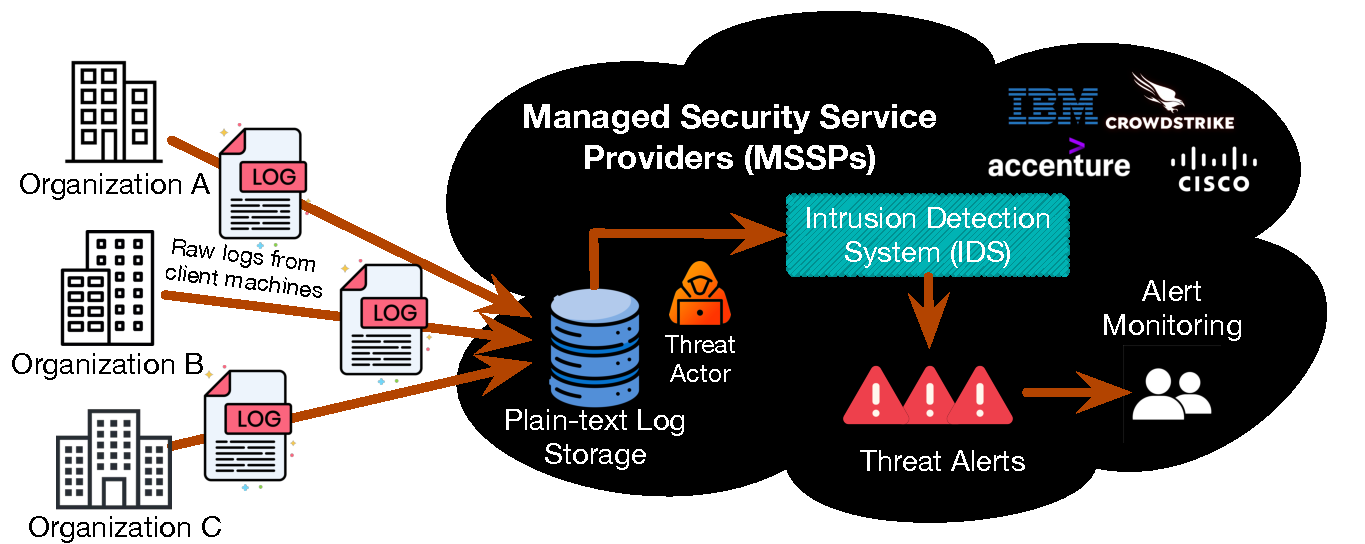
\includegraphics[width=0.35\textwidth]{fig/mssp.pdf}
  \caption{The MSSP architecture for intrusion detection, which is vulnerable to privacy leakage. The plain-text system logs are first collected in a centralized storage managed by the MSSP. Then these system logs are analyzed for intrusions.}
  \label{mssp}
  \vspace{-4ex}
\end{figure}

Recently, Provenance-based IDS (PIDS)~\cite{streamspot,provdetector2020,wang2022threatrace,shadewatcher,yangprographer,han2020unicorn} have emerged as a highly effective means of enhancing intrusion detection. These systems leverage the extensive contextual information provided by \logs to bolster their detection capabilities. PIDS operates by converting \logs into provenance graphs, which are then analyzed using machine learning techniques, such as Graph Neural Networks (\gnnshort), to identify and learn patterns of benign activity. By continuously monitoring these patterns, PIDS can detect deviations that may indicate potential security threats. Upon detecting such anomalous graph patterns, the PIDS generates alerts to prompt further investigation.


\subsection{Limitations of Existing PIDS}

Despite PIDS potential, the current operational mode of MSSPs and the state-of-the-art PIDS face significant challenges in the complex landscape of enterprise security, which are described below.

\smallskip
\noindent
\textbf{Privacy Risks and Centralized Dependency.} Current PIDS rely on a centralized infrastructure where client machines transmit their logs to a central server. While this centralization is necessary for aggregating large datasets to effectively model and understand benign behaviors using advanced deep learning techniques, it raises significant privacy concerns. Logs often contain sensitive information, such as URLs visited, IP addresses, and application usage, which can be exposed in centralized systems. These privacy risks are not merely theoretical; they have been highlighted in a recent Datadog report~\cite{datadog}. Additionally, training models on data from a single machine is insufficient, as shown by our experiments with \flash on the DARPA OPTC dataset~\cite{darpaoptc}, where performance dropped by 40\% in F-score when using single-host data compared to multi-host data.

    
\smallskip
\noindent
\textbf{Scalability and Operational Inefficiencies}  Centralized PIDS face significant challenges related to both network overhead and scalability. Transmitting large volumes of logs over the network for intrusion detection imposes substantial costs on users and organizations. Modern systems can generate gigabytes of logs daily~\cite{inam2023sok,hossain+depend}. Our analysis of PIDS, such as \flash and \kairos, using the \optc dataset as detailed in Section~\ref{cost_metric}, highlights this issue. For organizations similar in scale to those in the \optc dataset, daily log volumes can reach 1000 GB. This leads to considerable network expenses and difficulties for users with limited bandwidth who struggle to upload such large amounts of logs efficiently. As the number of hosts within an organization increases, centralized PIDS often experience log congestion, creating bottlenecks that slow down intrusion detection. Centralization also results in significant disk storage overhead, requiring continuous resource allocation to manage the growing data. Our evaluations of \flash and \kairos show that these systems would face severe log congestion in environments comparable to the \optc dataset. \flash would require 27.7 hours and \kairos 56.6 hours to process a single day's logs, highlighting the lack of scalability in current centralized PIDS solutions.


\subsection{Our Approach \& Contributions}

To address these challenges, we introduce \Sys, a novel privacy-preserving PIDS that integrates provenance graph representation learning with Federated Learning (FL). In \Sys, client logs remain local, which significantly enhances user privacy by ensuring sensitive data does not leave the client's environment. Each client independently trains \gnnshort models, and these models are aggregated on a central server with those from other clients, capturing diverse activity patterns across organizations without transmitting actual logs, thus minimizing network overhead. Instead, the only data transmitted are model updates, which are mere kilobytes per client, significantly reducing the network burden. All major computations, including the training and operational phases of \Sys, take place locally on client machines, using their computing resources to process provenance graphs derived from their logs for real-time threat detection. This approach allows \Sys to scale effectively with the addition of more hosts, each utilizing its own computing power and storage, addressing scalability and efficiency comprehensively.

The implementation of FL for a privacy-preserving PIDS introduces multiple challenges. Firstly, model aggregation in a federated setting becomes complex due to heterogeneous data distributions~\cite{qu2022rethinking} from clients running different applications, leading to suboptimal unified model performance. Additionally, data imbalances~\cite{duan2020self} across clients, where smaller data contributors have less impact on the federated model, skew the learning outcomes. Another significant hurdle is the inconsistent semantic information produced by independently trained \wordvec models on different client machines. This feature space inconsistency~\cite{zhou2023fedfa} across semantic encoders complicates the effectiveness of the global \gnnshort models, resulting in inaccurate system behavior representations due to varied feature vector qualities.

To effectively address the challenges of heterogeneity and data imbalance, we have designed a novel ensemble learning framework. In this framework, each submodel is trained to specialize in learning system activities associated with specific process entities, which are standardized across all clients. This standardization is facilitated by a sophisticated categorization scheme enabled by our dual-server architecture. Through this system, process entities from all clients are organized into \textit{K} privacy-preserving bins. Each client then aligns its process nodes with these bins, constructs a provenance subgraph for each bin, and trains a \gnnshort model on these graphs. The models from all clients are then aggregated into \textit{K} model pairs, forming a comprehensive global ensemble model set. This strategic approach ensures that models with similar data distributions are merged effectively, thereby maintaining the integrity of unique activity patterns across diverse client environments.

To address semantic inconsistencies in \wordvec models, we implement a \wordvec harmonization scheme utilizing a dual-server architecture. In this setup, a central server issues encryption keys to clients, allowing them to securely encode \wordvec tokens. Subsequently, a utility server processes these encrypted tokens to achieve a unified, privacy-preserving vector representation. This method ensures that sensitive data remains protected while facilitating accurate and consistent semantic encoding across different clients.

We have conducted extensive evaluations of our system's effectiveness using open-source datasets from \darpa, specifically E3~\cite{error3}, E5~\cite{bug5}, and \optc~\cite{anjum2021analyzing}. These datasets encompass a broad spectrum of attack scenarios and system behaviors. Our findings indicate that \Sys achieves high detection performance, with an average precision of 96\% and recall of 97\%. Thus, our system performs comparably to state-of-the-art centralized systems like \flash and \kairos. As detailed in section~\ref{cost_metric}, our system achieves a 170-fold reduction in communication and storage costs compared to \flash and \kairos. Since our technique is decentralized, our inference time is bounded by the client with the most log data; it will only take approximately 3 minutes to run inference on the complete \optc dataset, whereas \flash and \kairos take many hours.  We present a detailed analysis of the privacy protection of our system in Section~\ref{privacy}. We also provide a comprehensive analysis of our system's resilience against adversarial attacks in Section~\ref{sec:discussion}.

The main contributions of our work are as follows:

\begin{itemize}[topsep=.1ex,itemsep=-.1ex,leftmargin=*]
    \item[--] To the best of our knowledge, we are the first to introduce federated provenance graph learning in the domain of IDS with our system, \Sys.
    \item[--] We have introduced a novel \textbf{ensemble learning} and \textbf{process entity categorization} framework for dealing with diverse heterogeneous client data distributions.
    \item[--] We developed a sophisticated \textbf{\wordvec harmonization framework} using a multi-server architecture for secure private aggregation of semantic attributes.
    \item[--] We conduct a comprehensive evaluation of our technique on real-world datasets, demonstrating \Sys's effectiveness in detecting system threats while being scalable and privacy-preserving.
\end{itemize}

\PP{Availability.} We plan to open-source our codebase upon publication to promote further development in privacy-preserving IDS research. %\url{https://anonymous.4open.science/r/TrustWatch}

% \begin{table}[t!]
%   \centering
%   \scriptsize
%     %\caption{Limitations of existing PIDS. \wajih{Add in caption that which PIDS are not specified in the table and why.}}
%     \caption{Existing PIDS limitations. \flash and \kairos outperform other existing PIDS systems ~\cite{wang2022threatrace,han2020unicorn,streamspot,yangprographer,shadewatcher,provdetector2020}. Also, they all suffer from data privacy leakage issues. Therefore, we have excluded these PIDS from the table. }
%     \setlength{\tabcolsep}{10pt}
%       \begin{tabular}{ | c | c | c | c |}

%         \hline
%              & \bf Data & \bf Network  & \bf Scalability \\
%              & \bf  Privacy & \bf  Overhead &  \\
%         \hline
%         \hline
%         \disdet~\cite{dong2023distdet} & NO                       & LOW      & HIGH       \\
%         \hline
%         \flash~\cite{flash2024}     & NO            & HIGH             & MEDIUM      \\
%         \hline
%         \kairos~\cite{cheng2023kairos}     & NO            & HIGH             & LOW         \\
%         \hline
%         {\bf\Sys}  & YES                & LOW               & HIGH        \\
%         \hline
%       \end{tabular}
%       \label{tab:limitations}
%   \end{table}
